\section{Evaluation isolates the incremental output benefit}
\label{sec:protocol}

The comparison of interest is against tuned input-only MuonT. Its remaining loss gap is a few millinats, so learning-rate selection and numerical execution differences can be as large as the effect being measured. We use paired data ordering, an identity-factor execution control, and learning-rate sweeps at the full training budget before testing transfer.

\subsection{Models, budgets, and held-out losses}
\label{sec:testbed}

We train 32-layer, pre-RMSNorm SwiGLU Transformers on a 25.4B-token DCLM, StarCoderData, and Proof-Pile-2 mixture using the Marin PyTorch suite~\citep{mohamadi2026toner}. Runs use the Llama-3.1 vocabulary of 128,256 tokens, sequence length 4,096, document-isolated causal attention, and NVIDIA A100-40GB GPUs. Within each seed, optimizer arms share initialization and data ordering. The labels 130M and 520M refer to approximately 134M and 537M non-embedding parameters (\Cref{tab:regimes}).

\begin{table}[tbp]\centering\small
\setlength{\tabcolsep}{5.8pt}
\caption{\textbf{Pretraining regimes.} Params counts non-embedding parameters; TPP is tokens per non-embedding parameter. Fresh-seed confirmation uses seeds 1--3 after learning-rate selection and execution-path checks on seed 0.}\label{tab:regimes}
\begin{tabularx}{\textwidth}{@{}>{\raggedright\arraybackslash}Xrrrrrc@{}}
\toprule
Regime & Params & $\dm$ / $\dff$ & Tokens (TPP) & Batch / Steps & GPUs & Seeds \\
\midrule
130M controls \& LR bracket & 134M & 512 / 2,048 & 2.68B (20) & 0.5M / 5,120 & 8$\times$A100 & 0 \\
130M confirmation & 134M & 512 / 2,048 & 2.68B (20) & 0.5M / 5,120 & 8$\times$A100 & 1, 2, 3 \\
130M longer training & 134M & 512 / 2,048 & 10.74B (80) & 0.5M / 20,480 & 8$\times$A100 & 0 \\
520M width transfer & 537M & 1,024 / 4,096 & 10.74B (20) & 1.0M / 10,240 & 32$\times$A100 & 0 \\
\bottomrule\end{tabularx}
\end{table}


We report held-out training-mixture cross-entropy $\Lsel$, C4 loss $\Lc$, and the unweighted macro average over 16 Paloma domains $\Lpal$. Final losses measure completed models; paired means over 11 second-half checkpoints assess whether a difference persists through late training. Checkpoints from one trajectory are correlated observations and do not substitute for independent seeds. Figures report differences in millinats, where one millinat is $10^{-3}$ nats and negative differences favor the proposed method.

\subsection{Execution-path and learning-rate controls}
\label{sec:falsification}

Null-WT performs synchronous output capture, pooling, and root construction, then applies identity output factors. It controls the added numerical and collection path; it does not separately isolate asynchronous scheduling. It tests whether changes in tensor batching and mixed-precision accumulation can account for the measured gain. At learning rate 0.02263, its final loss is 0.0003 nats below MuonT, compared with a 0.0043-nat improvement for WT-MLP-Lag (\Cref{tab:controls}). The control makes execution-path drift an unlikely explanation for the full effect, although it is one measured control rather than a proof of numerical equivalence.

\begin{figure}[t]
 \centering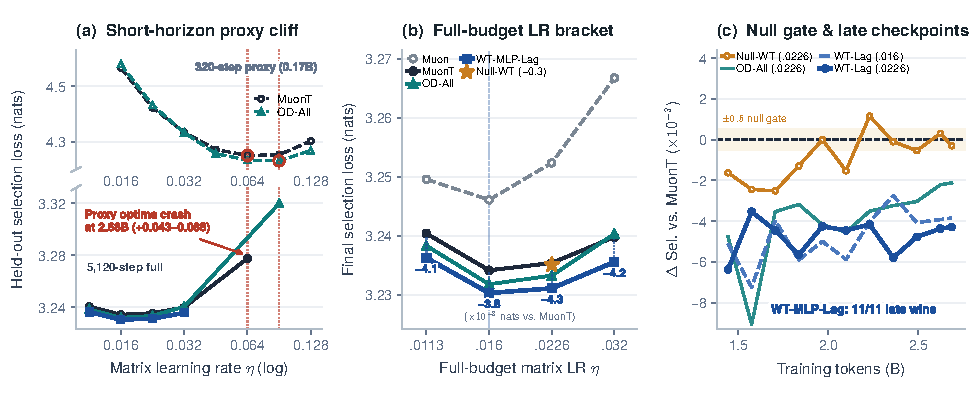
\includegraphics[width=\textwidth]{fig4_confounds_lr_null.pdf}
 \caption{\textbf{The gain survives full-budget tuning and an execution-path control.}
 \textbf{(a)} Learning rates selected on a 320-step schedule transfer poorly to the full budget.
 \textbf{(b)} Full-budget held-out loss across a learning-rate bracket, with a matched-path identity-factor control (Null-WT).
 \textbf{(c)} Late-training differences from MuonT at learning rate 0.02263: the control stays much closer to MuonT than WT-MLP-Lag does. All panels use 130M, seed 0; the full budget is 2.68B tokens.}
 \label{fig:confounds}
\end{figure}

\begin{table}[tbp]\centering\small
\setlength{\tabcolsep}{5.2pt}
\caption{\textbf{Seed-0 learning-rate bracket, execution-path control, and short-schedule transfer at 130M (2.68B tokens).} Entries are final held-out losses in nats across the complete four-point bracket (bold marks each row's full-budget minimum, $\eta^*=0.0160$ for every method); $\Delta_{0.0226}$ is the paired difference from MuonT at $\eta=0.02263$ in millinats where Null-WT is evaluated. The rightmost column transfers each checked arm's 320-step argmax learning rate (\Cref{tab:lr_cliff}) to the full 5,120-step schedule.}\label{tab:controls}
\begin{tabularx}{\textwidth}{@{}>{\raggedright\arraybackslash}Xrrrrrr@{}}
\toprule
& \multicolumn{4}{c}{Full-budget held-out loss $\Lsel$ (nats)} & & \\
\cmidrule(lr){2-5}
Method & $0.0113$ & $0.0160$ & $0.0226$ & $0.0320$ & $\Delta_{0.0226}$ (mnats) & 320-step $\eta^* \to$ full \\
\midrule
Muon & 3.2496 & \textbf{3.2461} & 3.2524 & 3.2667 & $+16.96$ & --- \\
MuonT & 3.2404 & \textbf{3.2342} & 3.2354 & 3.2398 & $+0.00$ & $0.0640 \to 3.2775$ \\
Null-WT (ctrl) & --- & --- & 3.2351 & --- & $-0.30$ & --- \\
OD-All & 3.2383 & \textbf{3.2318} & 3.2333 & 3.2403 & $-2.13$ & $0.0905 \to 3.3200$ \\
\rowcolor{rowtint}[0pt][0pt]\textbf{WT-MLP-Lag} & 3.2363 & \textbf{3.2303} & 3.2311 & 3.2356 & $\mathbf{-4.29}$ & --- \\
\bottomrule\end{tabularx}
\end{table}


Learning rates selected on a short schedule do not transfer reliably to the full budget. A 320-step sweep favors rates of 0.064--0.0905, three to four times the useful full-budget scale. Transferring those choices to 5,120 steps worsens final loss by 0.04--0.09 nats in the checked arms, overwhelming the output-side gain. This is consistent with broader concerns about optimizer comparisons across tuning budgets and horizons~\citep{choi2019empirical,schmidt2021crowded,kaddour2023nodata,dang2026batchsize}.

We therefore sweep $\eta\in\{0.01131,0.016,0.02263,0.032\}$ across all four core methods at the full 2.68B-token budget (\Cref{fig:confounds}(b),\Cref{tab:controls}). Every method achieves a strict interior minimum at $\eta^*=0.016$, rising on both the cooler ($\eta=0.01131$) and hotter ($\eta\ge0.02263$) sides, while WT-MLP-Lag improves on MuonT at every matched rate by 0.0038--0.0043 nats. Sharing the same full-budget optimum allows fresh-seed confirmation across all four methods at a common learning rate without schedule confounds; we also record the hotter $\eta=0.02263$ replicates for OD-All and WT-MLP-Lag in \Cref{app:appendix_lr}.
